% This is samplepaper.tex, a sample chapter demonstrating the
% LLNCS macro package for Springer Computer Science proceedings;
% Version 2.20 of 2017/10/04
%
\documentclass[runningheads]{llncs}
%
\usepackage{graphicx}
\usepackage{url}
% Used for displaying a sample figure. If possible, figure files should
% be included in EPS format.
%
% If you use the hyperref package, please uncomment the following line
% to display URLs in blue roman font according to Springer's eBook style:
% \renewcommand\UrlFont{\color{blue}\rmfamily}

\newcommand{\Jupyter}{\textbf{Jupyter}}

\begin{document}
%
\title{Using the wonderful \Jupyter{} ecosystem and notebooks for teaching and practical sessions\thanks{Supported by ENS Rennes and CentraleSup{\'e}lec.}}
%
\titlerunning{Introduction to \Jupyter{} notebooks}
% If the paper title is too long for the running head, you can set
% an abbreviated paper title here
%
\author{Lilian Besson\inst{1}\orcidID{0000-0003-2767-2563}}
%
\authorrunning{Lilian Besson}
% First names are abbreviated in the running head.
% If there are more than two authors, 'et al.' is used.
%
\institute{{\'E}cole Normale Sup{\'e}rieure de Rennes, Bruz, France\\
\email{lilian.besson{@}ens-rennes.fr}\\
\url{http://www.ens-rennes.fr/}}
%
\maketitle              % typeset the header of the contribution
%
\begin{abstract}
    % https://www.didapro.org/8/contributions-dates/

    I propose a tutorial that will introduce the \Jupyter{} notebooks and give a good overview of the large \Jupyter{} ecosystem.
    I will explain and show how one can easily (and for free) use \Jupyter{} notebooks with the Python programming language, as well as other languages.
    Notebooks can be used for lecture material, to obtain one document that contains text, maths, figures, code snippets and the outputs of their execution.
    \Jupyter{} Notebooks are also an excellent tool to use for practical sessions in studying computer science, but also any other science with numerical computations or data analysis (mathematics, physics and chemistry, engineering etc), as a template or a skeleton can be given to the students, and collected and rated after the practical session.

    I illustrate this tools and present how to write clean and pretty notebooks, how to convert them to HTML, source code or PDF, by detailing my daily usage of the \Jupyter{} ecosystem as a professor of computer science at ENS de Rennes.
    I have used \Jupyter{} notebooks from L3 to M2 level since the last three years, and I want to share this expertise with other teachers of computer science.
    My documents are open-sourced and published online, and are used for a course on algorithms (L3), and for the training for the computer science major option at the ``agr{\'e}gation'' national exam in mathematics.

    % The abstract should briefly summarize the contents of the paper in 150--250 words.

\keywords{Jupyter \and Notebook \and Python \and Open-source tool \and Teaching programming \and Data science.}
\end{abstract}
%
%
%

% -------------------------
\section{Outline of the tutorial content}

In 30 minutes, and as many times as possible on the Wednesday 7th of February, the author proposes to present the following points.

\paragraph{Presentation of \Jupyter}

\begin{itemize}
    \item What is a \Jupyter{} notebook: a what-you-see-is-what-you-get (WYSIWYG) integrated development environment (IDE) for (almost) any programming language. For instance, it can be used for interpreted dynamic languages such as Python \cite{python}, OCaml\footnote{With \url{https://github.com/akabe/ocaml-jupyter}, and other ``kernels'' for other languages.}, Julia or Bash, but also compiled languages such as C/C++ etc.

    \item What is the \Jupyter{} ecosystem: it started as ipython \cite{ipython} about 20 years ago, designed to be used only for the Python programming language, and nowadays it has evolved into a mature open-source ecosystem.
    It is used by hundreds of thousands of scientists from all over the world, and among its recent successful uses, one can note the first ever picture of a black whole by Katie Bouman and collaborators\footnote{See for instance \url{https://www.nationalgeographic.com/science/2019/04/first-picture-black-hole-revealed-m87-event-horizon-telescope-astrophysics/} and \url{https://www.bbc.com/news/science-environment-47891902}.}, or by Nobel laureates such as Paul Romer\footnote{See \url{https://paulromer.net/jupyter-mathematica-and-the-future-of-the-research-paper/}}.
    Jupyter notebooks are a free and open-source alternatives to proprietary IDE included in MATLAB, Wolfram's Mathematica and MapleSoft's Maple software.

    \item What problems solve \Jupyter{} notebooks? Why they are awesome, both easy to learn and use for beginners and powerful for expert users.
\end{itemize}

\paragraph{How to install \Jupyter}

By following the online tutorial from \url{https://jupyter.org/install.html}, it is easy to install the entire \Jupyter{} ecosystem on any computer with Python and \texttt{pip} or \texttt{conda} installed.


\paragraph{How to use \Jupyter{} to write simple documents}

We will discover together the Graphical User Interface of \Jupyter{} notebooks, and learn how to write text, maths, code cells.
%
I will also show the official online tutorial and documentation, as pointers to learn by yourself.


\paragraph{Presenting my own usage of \Jupyter{} notebooks}

I will show how I have been using \Jupyter{} notebooks on a daily basis for my teaching activities, since the last three years.
I will mainly present examples of resource produced from a \Jupyter{} notebook, and how to convert notebooks to HTML.

\begin{itemize}
    \item
    Using the \textbf{OCaml} language,
    for the 3rd year (M2) students at ENS de Rennes,
    I used \Jupyter{} notebooks to write the sheets and solutions of practical sessions used for training our students for the ``modelisation'' oral exam of ``agr{\'e}gation'' nation exam.
    See \url{https://nbviewer.jupyter.org/github/Naereen/notebooks/tree/master/agreg/TP_Programmation_2017-18/}

    \begin{figure}[!h]
        \centering
        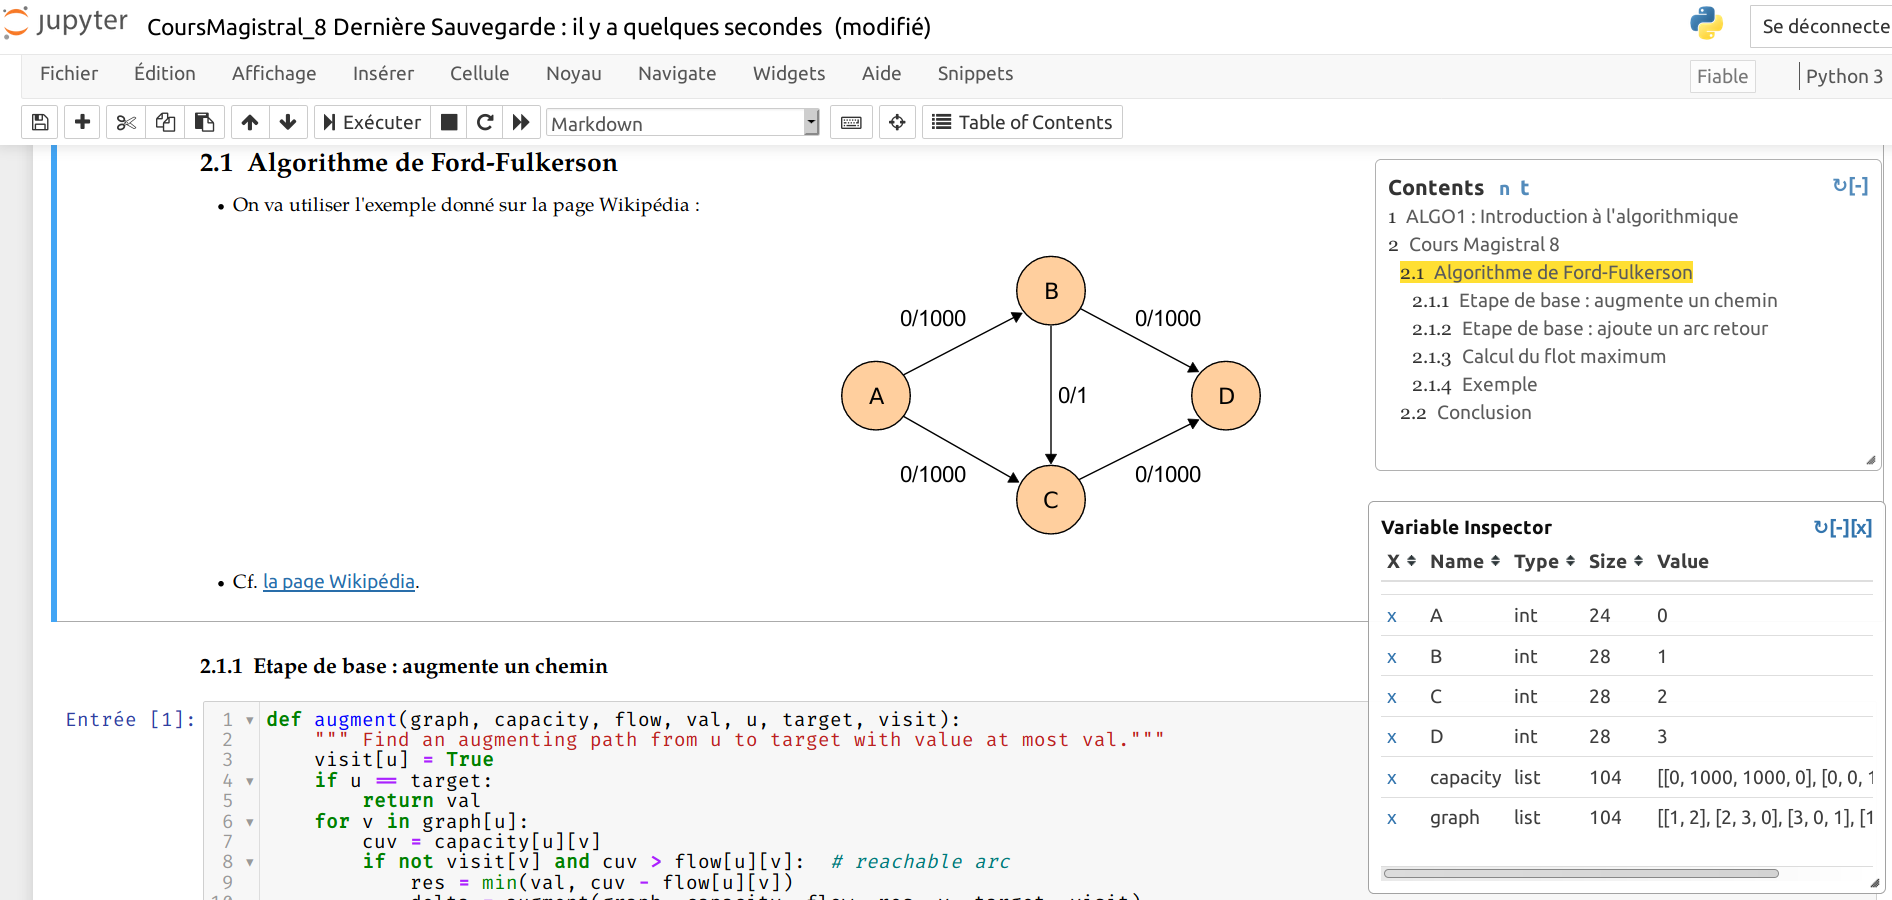
\includegraphics[width=10cm]{apercu_ENS_agreg_4.png}
        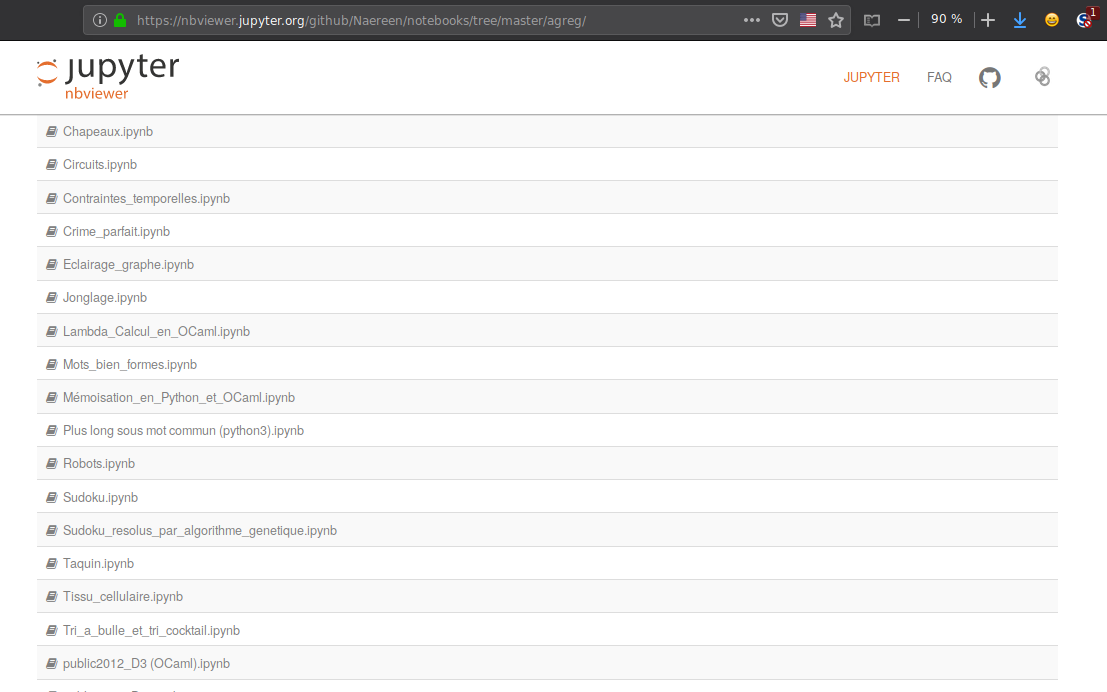
\includegraphics[width=6cm]{apercu_ENS_agreg_1.png}
        % 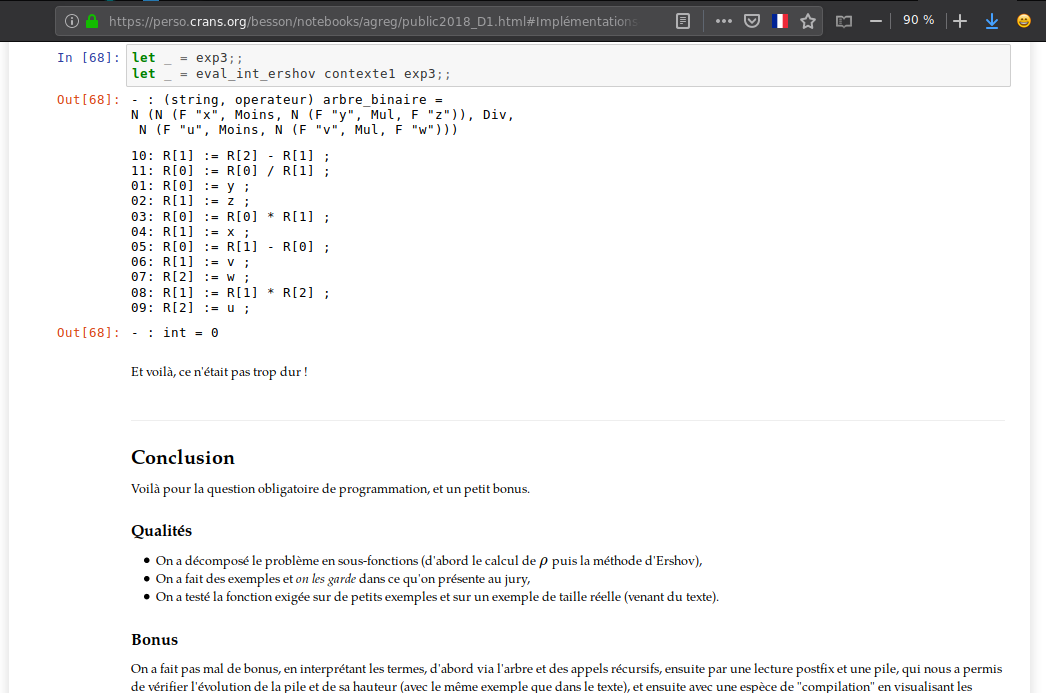
\includegraphics[width=6cm]{apercu_ENS_agreg_2.png}
        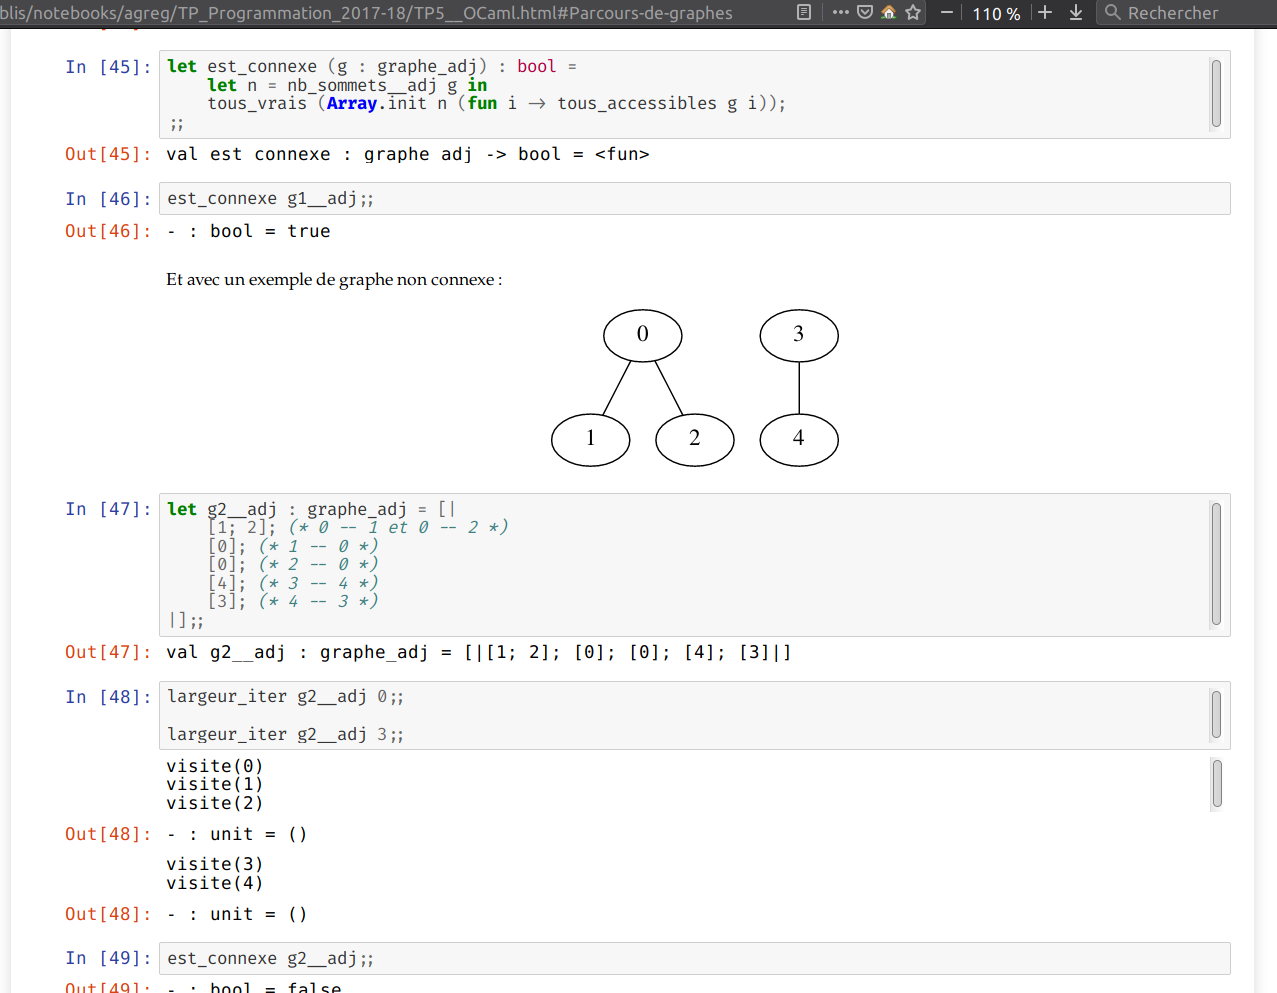
\includegraphics[width=6cm]{apercu_ENS_agreg_3.png}
        \caption{Examples of use of \Jupyter{} notebooks.}
        \label{}
    \end{figure}


    \item
    Using the \textbf{Python} language, for 1st year (L3) students at ENS de Rennes,
    I wrote a lot of clean and detailed implementations of data structures and algorithms from scratch, for my course on Algorithms in Autumn 2019.
    See \url{https://github.com/Naereen/ALGO1-Info1-2019/}

    \item
    Using \textbf{Python} and maths,
    for students in a PSI class (CPGE) at Lyc{\'e}e Joliot-Curie in June 2017 to 2019,
    I wrote the solutions for practical sessions given as training for the oral ``maths with Python'' exam in Jupyter notebooks, in order to share them easily with the students, and display and work on them during the practical sessions.
    See \url{https://perso.crans.org/besson/notebooks/Oraux_CentraleSupelec_PSI__Juin_2019.html}

    \item
    With a colleague, we gave a 1 hour tutorial introducing the Julia programming language, in yearly seminar of the IETR lab in June 2018 in Vannes, for about 50 people.
    We used two \Jupyter{} notebooks during the seminar \url{https://github.com/pierre-haessig/julia-presentation-ietr2018/},
    and these slides \url{https://hal.archives-ouvertes.fr/cel-01830248/}.

\end{itemize}



\paragraph{Pointers on how to become a \Jupyter{} expert}

I want to conclude the tutorial by giving links and ideas to master the \Jupyter{} ecosystem and use them for your own project.

\begin{itemize}
    \item How to use a GitHub/Bitbucket/GitLab repository to host \Jupyter{} notebooks, and display them online using the \url{https://nbviewer.jupyter.org/} website.
    See \url{https://github.com/Naereen/ALGO1-Info1-2019/} and \url{https://github.com/Naereen/notebooks/}
    \item Use Binder, Google Colab or other online free tools to add a link so that any user of your \Jupyter{} notebooks can start interactive environment directly from their web browser, to interact with the notebook.
    \item Use \Jupyter{} extensions to extend the IDE, for instance to automatically add a table of contents. See \url{https://jupyter-contrib-nbextensions.readthedocs.io/en/latest/}.
    \item Study from the masters, for instance the famous Peter Norvig publishes very interesting notebooks on his project \url{https://github.com/norvig/pytudes} since 5 years.
    \item Share your notebooks online, with your students and colleagues, and receive feedback from them!
\end{itemize}


% -------------------------
\section{Technical details}

We list the required materials for the tutorial, and other technical details.

\paragraph{Material}

\begin{itemize}
    \item Each participant must come with its own laptop.
    \item Bonus if the \Jupyter{} ecosystem is already installed.
    \item One large screen and projector.
\end{itemize}


\paragraph{Other details}

\begin{itemize}
    \item There are no limit in terms of number of how many people can attend this tutorial, except the limitation of the room.
    \item Note that no prior knowledge on the Python language is needed to use \Jupyter{} notebooks.
\end{itemize}



% -------------------------
\section{Practical session}

I will, of course, use a Jupyter notebook as the material displayed during the tutorial (so the talk itself is a meta-example).
For the people attending the seminar, and for curious people who would miss it, I will share the presentation notebook online beforehand.

The tutorial will also contain a ``homework'' for the interested people, as a notebook with blanks to fill and tasks to solve.
I will offer to review the filled notebook if anyone wants to send it to me, and offer a support by email if needed (even if StackOverflow does a much better job than anybody).


% ---- Bibliography ----
%
% BibTeX users should specify bibliography style 'splncs04'.
% References will then be sorted and formatted in the correct style.
%
% \bibliographystyle{splncs04}
% \bibliography{mybibliography}
%
\begin{thebibliography}{8}
\bibitem{jupyter}
Thomas Kluyver et al.
\textbf{Jupyter Notebooks - a publishing format for reproducible computational workflows}.
In F. Loizides and B. Schmidt, editors, Positioning and Power in Academic Publishing: Players, Agents and Agendas, pages 87–90. IOS Press, 2016.

\bibitem{python}
Python Software Foundation.
\textbf{Python Language Reference}, version 3.6, October 2017. \url{www.python.org}.

\bibitem{ipython}
Fernando Pérez and Brian E. Granger.
\textbf{IPython: a System for Interactive Scientific Computing}.
\emph{Computing in Science and Engineering}, 9(3):21–29, May 2007. ISSN 1521-9615. \url{ipython.org}.
\end{thebibliography}
\end{document}
